\documentclass[11pt]{article}
\usepackage{royden-report}
\usepackage[T1]{fontenc}
\usepackage{lmodern,microtype}
\title{Three complex initial envelopes}
\author{A bounded spatial Dysthe simulator demonstration}
\date{16 October 2026}
% Generated by stage2/plot_demo.py from checksummed frozen fields.
\newcommand{\DemoGaussianPeak}{1.406646}
\newcommand{\DemoGaussianShape}{39.31}
\newcommand{\DemoGaussianWidthChange}{0.0197}
\newcommand{\DemoProfileShape}{$2.77\times10^{-10}$}
\newcommand{\DemoProfilePhase}{-8.000000}
\newcommand{\DemoTotalSeconds}{106.3}
\newcommand{\DemoPeakRSS}{197.0}
\newcommand{\DemoFinalTable}{
\begin{tabular}{lrrrrr}
\toprule
Case & Peak & RMS width & Displacement & Shape & Tail fraction \\
\midrule
Reference profile & 1.958116 & 0.623359 & $-3.21\times10^{-10}$ & $2.77\times10^{-8}\%$ & $2.72\times10^{-10}$ \\
Localized perturbation & 2.018419 & 0.606491 & 0.054528 & 2.57\% & $4.96\times10^{-5}$ \\
Complex Gaussian & 1.325587 & 1.414492 & -1.936173 & 39.31\% & $6.22\times10^{-3}$ \\
\bottomrule
\end{tabular}}
\newcommand{\DemoConvergenceTable}{
\begin{tabular}{lrrrr}
\toprule
Case & Grid & Step & Domain & Domain orbital \\
\midrule
Reference profile & $4.17\times10^{-15}$ & $3.07\times10^{-9}$ & $1.54\times10^{-6}$ & $1.54\times10^{-6}$ \\
Localized perturbation & $3.09\times10^{-15}$ & $4.08\times10^{-9}$ & $2.26\times10^{-6}$ & $1.83\times10^{-6}$ \\
Complex Gaussian & $9.28\times10^{-16}$ & $4.05\times10^{-11}$ & $2.18\times10^{-5}$ & $9.66\times10^{-9}$ \\
\bottomrule
\end{tabular}}

\begin{document}
\maketitle
\vspace{-1em}
\section{Problem and prescribed inputs}
The simulator advances the scaled complex free-surface envelope $u(\xi,\tau)$,
where $\xi$ is propagation distance and $\tau$ retarded time:
\[
 u_\xi=-\mathrm{i}u_{\tau\tau}-\mathrm{i}|u|^2u
 -\epsilon\bigl(8|u|^2u_\tau+2u^2\overline{u_\tau}
                   +2\mathrm{i}u|D_\tau|(|u|^2)\bigr).
\]
The model contract is \texttt{water-wave-dysthe-spatial-v1}.
The coefficients are $(1,1,8,2,2)$.
The periodic interval is $[-80,80)$, $N=4096$, $\epsilon=0.025$,
$\Delta\xi=0.00125$, and $0\leq\xi\leq4$. There are 81 saved positions.
The Fourier method retains $|m|<N/4$, uses mean-flow symbol $|k|$ with zero
mean mode, and applies Lawson integrating-factor RK4.

Let $F$ be the recomputed periodic branch with $\mu=2$, $s=0$, and full
traveling residual $2.03\times10^{-11}$. The three initial fields are
$F(\tau)$; $F(\tau)[1+0.02\exp(-((\tau-1.3)/2)^2)]$; and
$\exp(-\tau^2/8)\exp(0.3\mathrm{i}\tau)$. The second is a shifted localized
amplitude perturbation. The third has amplitude 1, width parameter 2,
wavenumber 0.3, and zero chirp. The plots retain physical coordinates and
show envelope amplitude, rather than reconstructed surface elevation.

\begin{figure}[htbp]
\centering
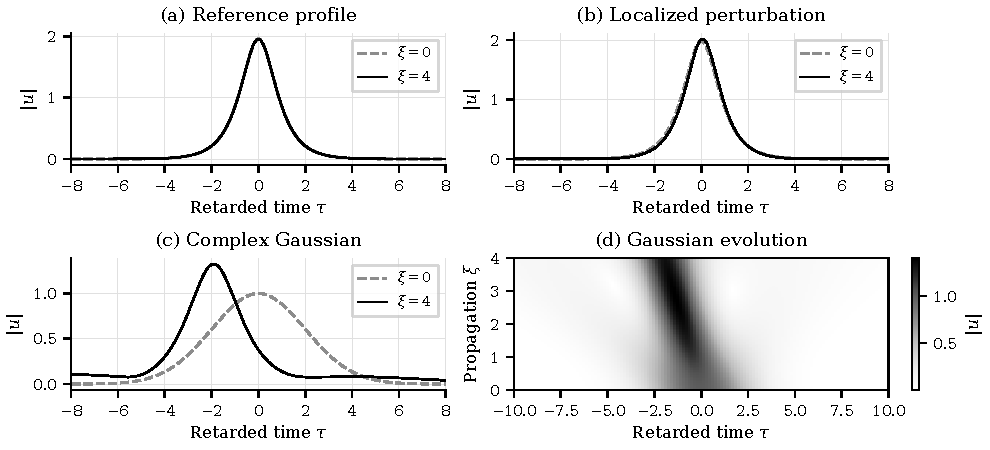
\includegraphics[width=\linewidth]{figures/envelopes.pdf}
\caption{Initial and final amplitudes for all three cases, and the Gaussian
trajectory. These are central-window views of the saved full-domain complex fields.}
\end{figure}
\clearpage

\section{Observed evolution}
The reference keeps its amplitude and width to the reported accuracy while
its fitted global phase changes by $\DemoProfilePhase$ radians. Its final
shape distance is \DemoProfileShape. The perturbed profile deforms modestly
and develops exterior action. The Gaussian focuses to maximum amplitude
$\DemoGaussianPeak$ and ends at amplitude 1.325587. Its final shape distance
is $\DemoGaussianShape\%$ despite a net width change of only
$\DemoGaussianWidthChange\%$. Width alone therefore misses substantial
complex-envelope evolution.

\begin{figure}[htbp]
\centering
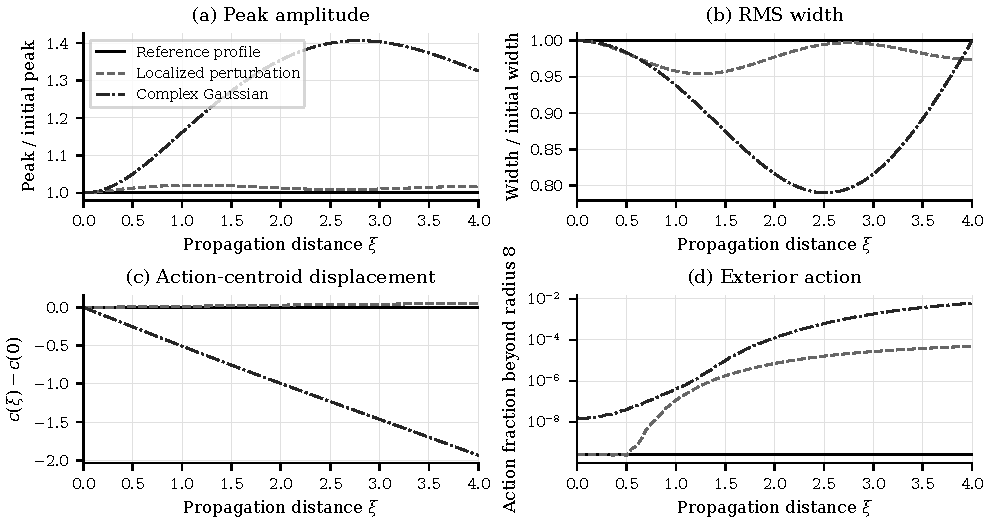
\includegraphics[width=\linewidth]{figures/metrics.pdf}
\caption{Peak and width relative to their own initial values; action-centroid
displacement; and action beyond periodic distance 8 from that centroid.
The exterior fraction includes packet tails and spreading and is not automatically radiation.}
\end{figure}

\begin{table}[htbp]
\centering
\small
\caption{Final values at $\xi=4$. Shape is the relative complex L2 distance
to each case's initial field after removing translation and constant phase,
without amplitude rescaling.}
\DemoFinalTable
\end{table}

The centroid is obtained from the first circular action moment; displacement
is unwrapped relative to its initial value. RMS width is the action-weighted
shortest periodic distance about that centroid. These statistics become
ambiguous for broad or wrapped fields. Here circular concentration remains
above 0.998. The complex shape diagnostic also detects phase variation that
amplitude plots cannot show.
\clearpage

\section{Numerical qualification and reproducibility}
Each default case has independent comparisons with $N=8192$ at fixed domain,
$\Delta\xi=0.000625$ at fixed grid, and $(L,N)=(320,8192)$ at fixed spacing.
All nine comparisons and the recorded design screens pass. Profiles are
recomputed for each period. The table reports maxima over all 81 saved
positions, retaining complex phase in the raw comparisons.

\begin{table}[htbp]
\centering
\small
\caption{Maximum relative complex L2 differences. Domain comparisons use
common physical coordinates in the central $[-80,80)$ window. The last
column additionally removes translation and constant phase.}
\DemoConvergenceTable
\end{table}

The raw-field normalization is the refined field norm at each position.
The chosen gates are $2\times10^{-4}$ for raw differences and $10^{-4}$ for
orbital differences and signed-shape discrepancies. The latter compare each
solution's deformation from its own initial field. Their additional relative
response gate is $0.02$, used only above a $10^{-7}$ field-norm response floor.
The tiny reference response falls below that floor. Two levels demonstrate
agreement; they provide neither an observed convergence order nor a rigorous
error bound. Periodic mean flow can depend on $L$ even when boundary action
is tiny; domain differences include that dependence.

Signed-shape comparisons can have an approximately $10^{-8}$ fitting floor
under the inherited orbital optimizer even when raw grid differences are
near $10^{-15}$. This is a diagnostic precision limit, not evidence of an
unresolved propagated field. Action conservation is supporting evidence;
padded continuum energy and momentum are not assumed exact invariants of
the projected equation or RK map.

The stored arrays \texttt{tau}, \texttt{xi}, \texttt{u}, and \texttt{initial}
are available in each case's \texttt{fields.npz}; \texttt{u} is complex128 of
shape $(81,4096)$. Reports record parameters, definitions, qualification,
source hashes, and field checksums. Plotting verifies those checksums and
metadata against the saved summary before reading the fields. The completed
12-trajectory campaign, including refinements, used \DemoTotalSeconds\ seconds
of solver/diagnostic time and peak process RSS \DemoPeakRSS\ MiB.

From the task root, reproduce these plots and tables without rerunning propagation:
\begin{verbatim}
python3 stage2/plot_demo.py
cd stage2/report
pdflatex -interaction=nonstopmode -halt-on-error report.tex
pdflatex -interaction=nonstopmode -halt-on-error report.tex
\end{verbatim}
The plot manifest, source data, and earlier numerical-reference report are:
\begin{flushleft}
\small
\path{stage2/results/plot-manifest.json}\\
\path{stage2/results/demo/}\\
\path{stage2/review/dysthe-stage-one-reference.pdf}
\end{flushleft}

These checks qualify only the exact three defaults and $\xi\in[0,4]$.
Custom parameters and longer horizons require their own refinements. This
small simulator demonstrates varied complex initial envelopes and preserves
their full fields; it establishes no soliton discovery, stability theorem,
Euler-model validation, training dataset, or learned operator.
\end{document}
